% Chapter 6
\chapter{Benchmarking and Life Cycle Cost Evaluation} % Write in your own chapter title
\label{Chapter6}
\lhead{Chapter 6. \emph{Benchmarking and Life Cycle Cost Evaluation}} % Write in your own chapter title to set the page header
In this chapter, a benchmarking approach by employing the exponential hazard model discussed in Chapter \ref{Chapter2} and mixture hazard model detailed in Chapter \ref{Chapter4} will be presented. The core objective of benchmarking approach is to search for the best practices in all facets of asset management. Particularly, focuses of this Chapter will be on pavement system. Needless to say, benchmarking approach can be widely applicable for all kinds of infrastructure as a whole. In view of hazard model and life cycle cost analysis, benchmarking approach is proposed for defining the best possible design and construction technology. In addition, the best practices in maintenance and repair can also be further discussed. If benchmarking approach is employed, it can facilite the standarlization of design, construction, maintanance and repair. This chapter will extensively discuss the integration approach between life cycle cost model and Markov hazard model. Empirical study will be conducted to simulate its application on pavement management system in Vietnam.
%%%%%
\section{General introduction}
\label{61}
The word benchmarking first known in 1980s when The Rank Xerox, a reputation company with specialize in manufacturing copiers found in 1959, introduce for improving its operations to be more advance competitive against its competitor. With applying properly the concept and practice of benchmarking, Rank Xerox had gained remarkable success during that time. In addition, it had paved a strong fundamental background for its continuous development. As the result, benchmarking concept and practice spreads from manufacturing sector to other business sectors today, including construction project management and infrastructure asset management.

Asking for the life cycle cost analysis, suffice to say, it becomes extremely important in today selection for business cycle as well as for infrastructure planning, which include selection for infrastructure investment, fiscal budget allocating for maintenance and repair. Since the public infrastructure requires a great allocation of resources, thus economic evaluation would become one of the blackbone tool. Together with benchmarking approach, it is hope that the methodology of this chapter would significantly bring a new dimension for continously improvement in infrastructure asset management.

We now further discuss the benchmarking and life cycle cost for pavement management system as for a general case. In actual situation, the quest for selection of best pavement technology, particularly based on material, structure and construction technique, is realized in high attention, especially in developing nations \cite{kcleong}. A good example is the national road system in Vietnam, where the entire road system is comprised of many different technologies. Reason to this is, as the matter of fact, due to limited capacity, the country often borrowed technologies from abroad. National standards for design and construction practices are somewhat mimic versions of guidelines, most of them are copied from developed nations. This practice is definitely unlike to that of developed nations. Consequently, leads to huge amount of efforts and budget in monitoring and maintenance during operation phases. Hence, in view of long term and strategic management, there is a strong demand in searching for the best pavement technology, which could become a national standard in pavement management system.

Selection for the best technology is thereby, having a close link to benchmarking study, which, as a must, depending on performance of road measured by simulation of deterioration hazard model. However, since the road infrastructure system comprising of many groups categorized by technological differences, the overall degradation of entire system is generally in average value, which largely depends on the deterioration speed of individual group. Each group is regarded as distinguished technological fashion characterizing by its heterogeneity factor. Thus, returning to the target of benchmarking study, it is necessary to develop a analytical approach to estimate the heterogeneity factor in order to reveal the deterioration progress of respective pavement technology.

A recent study on risk management in pavement system using mixture model has attracted attention for benchmarking study on pavement management system \cite{namieee}. This study employed Markov chain model for estimation of hazard rate and transition probability. However, it remains some limitation such as: a full scale of benchmarking study was not targeted. Further, empirical study only focused on a small numbers of samples. Thus, the aim of this chapter is to propose a fully description of methodology for benchmarking purposes. 

%%%%%%%
\section{Benchmarking-A proactive Approach in Infrastructure Management}
\label{62}
There are numerous definition on benchmarking, as a matter of fact, depending on where it is applied. In infrastructure asset management, the term benchmarking in asset management can be understood as a systemic and continuous measurement process or a process of continously measuring and comparing the practices within the system and against practices elsewhere in the world to gain information which will help existing system to improve its performance in the long run \cite{karlof}. A example in pavement management is a comparision of pavement technologies to find out the most suitable to local environment. In this sense, benchmarking can be defined to apply in various facets of asset management, from manegerial practices to technological selection. To summarize the basic philosophy of benchmarking, we summarize the approach in Figure \ref{fig61}.

%%
\begin{figure}[t]
\begin{center}
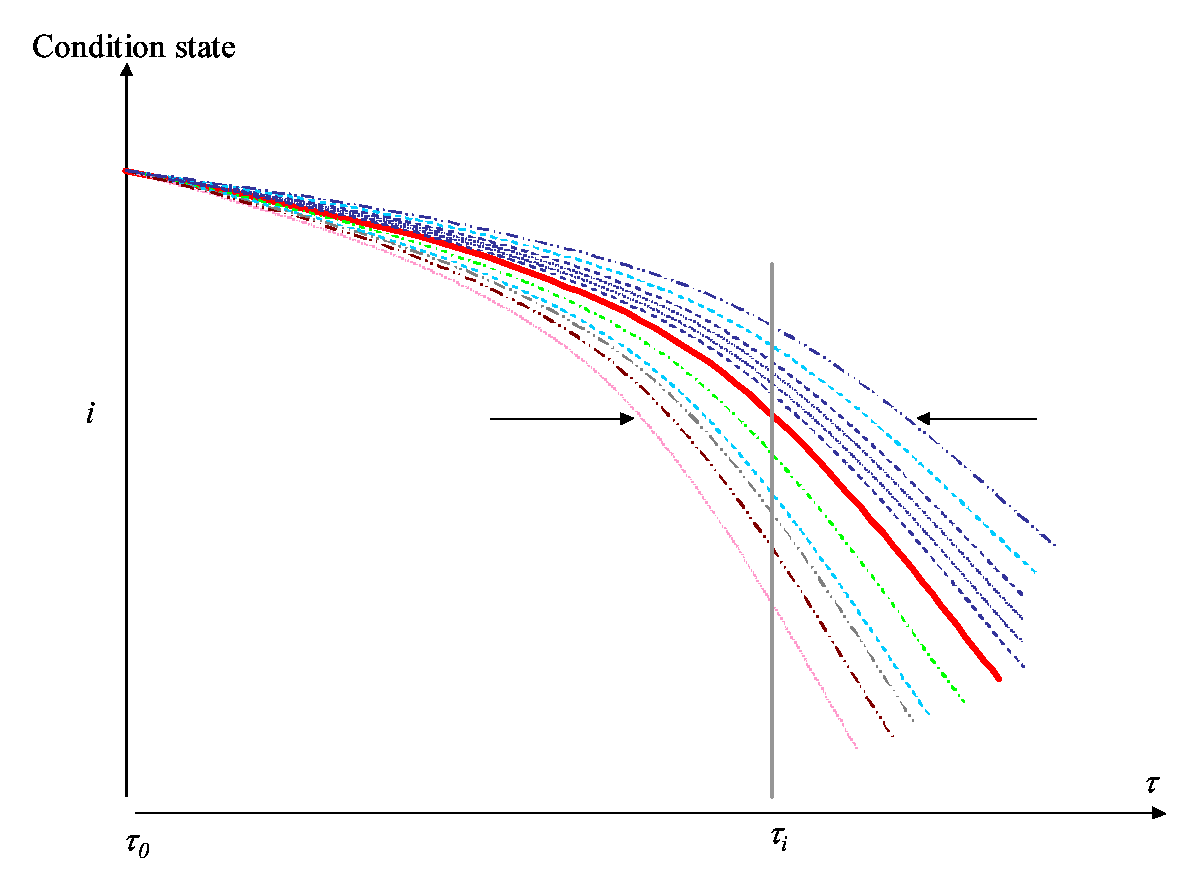
\includegraphics[scale=0.5]{fig61} 
\end{center}
\caption{Benchmarking objectives}
\label{fig61} 
\end{figure}
%%
With reference to hazard model developed in Chapter \ref{Chapter4}, it is realized that mixture model is best in describing the bahavior of individual group of infrastructure component, or road sections in our example case. By defining the objective of management, we are able to set up the target group of road sections, and thus, it is possible to relatively compare the deterioration of each group. In turn, it ought to be linked with objective of benchmarking study. Based on the methodology proposed in previous sections, we summarize the road map of benchmarking application in pavement management system in Figure \ref{fig62} . It is noted that cost evaluation technique is simply by comparing the average summary of construction and repairing cost when the condition state of road section entering the abosrbing state. Extension of cost evaluation technique using Markov decision theory can be further integrated into the model. However, it is out of the scope of this study. A simplified cost evaluation can give a good comparision of life cycle cost among the pavement technology. 

\begin{figure}[t]
\begin{center}
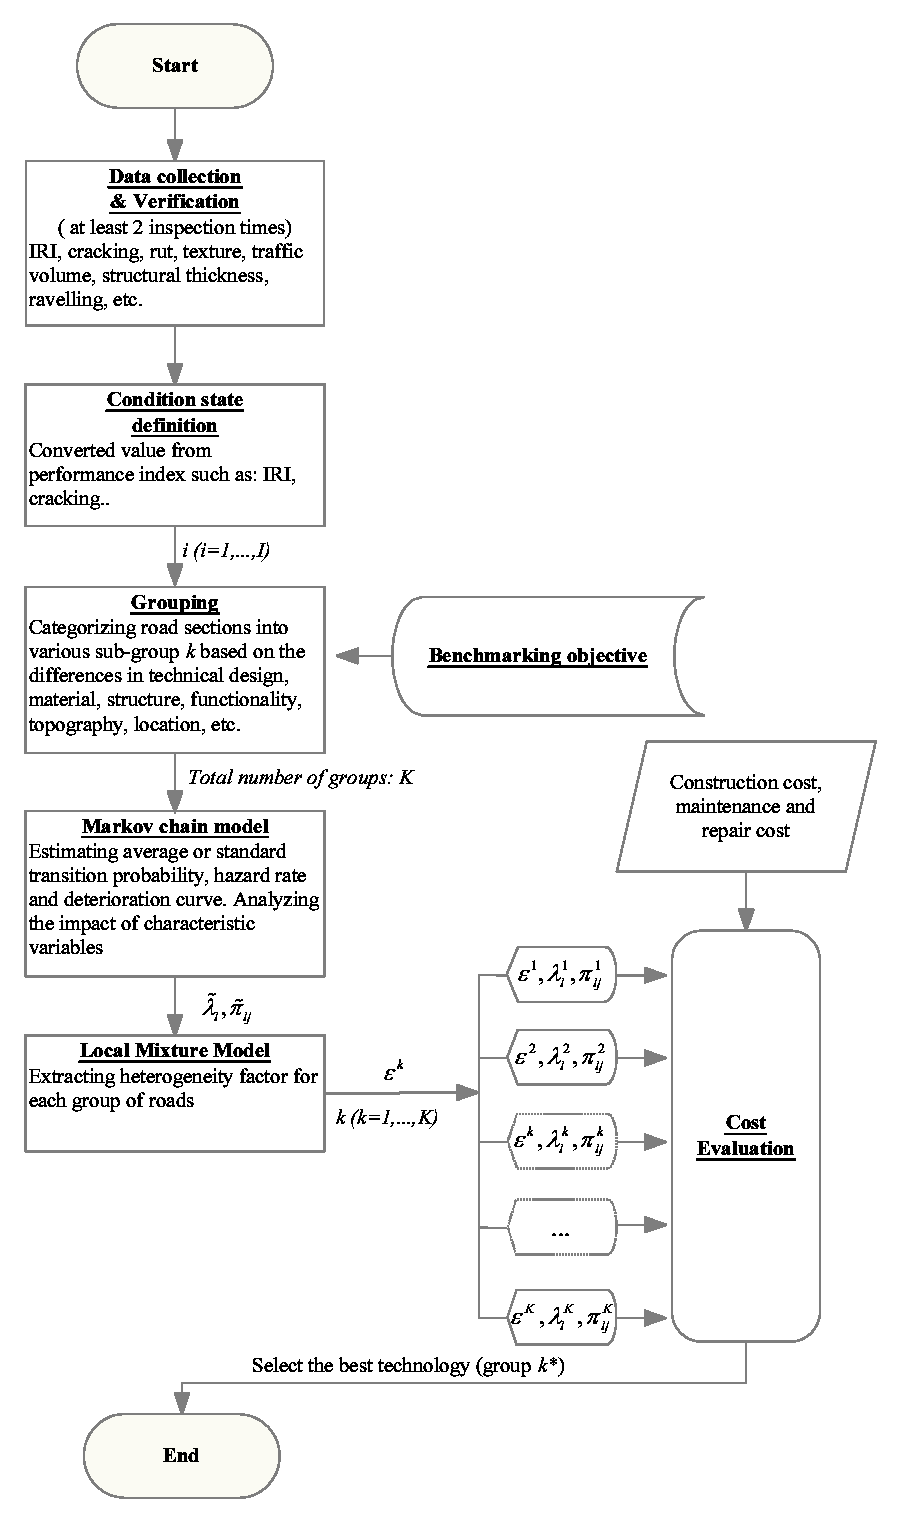
\includegraphics[scale=0.5]{fig62}
\end{center}
\caption{Benchmarking flowchart in PMS}
\label{fig62} 
\end{figure}
%
\section{Life Cycle Cost Evaluation For Infrastructure Management}
\label{63}
In section \ref{62} of this chapter, emphasis is solely on benchmarking approach to find the best possible pavement technology, which deems to be the scope of development phase when there exists the need to select the technolgy. Moreover, the economic evaluation methodology only assume a single renewal cycle rule. Needless to say, by use of that approach, at macroscopic view or network level, the model can give a good advice for decision maker. 

However, the life cycle cost technique based on that simple principle might not be highly recommeded when a project based analysis is considered. At project level, the task of management will largely focus on seeking for the best maintenance and repair. Thus, life cycle cost at project level should emcompass all possible M\&R technologies. 

Within the framework of benchmarking study, it is here again realized that benchmarking approach can assist us in finding out the best possible M\&R actions which exerts to have minimum life cycle cost and exhibits a sustainable practices. The course of life cycle cost at this level concerns two different methodologies (discount analysis and average cost analysis), which herein detailly presented.
%%%%%%%%
\subsection{Repair Action and Markov Transition Probability}
\label{631}
From previous Chapter, we categorize the condition of infrastructure into $K$ discrete states. $i$ is referred as condition state $i(i=1,...,K)$, and $t$ is management term to be set in an infinite state $t = (0, 1, .....)$. It is assumed that the repair action is carried out just before time $t$ when the condition state has already been determined by visual inspection. Repair action can be plural since it depends on various technologies. Here, let define $d\in D$ as a serial of rule that specifies the repair action, and $\eta^d(i) \in \Theta(i)$ as implemented repair action which change the condition state from $i$ to $j$, in another way $\eta^d(i) =j$. $\Theta(i)$ is a set of repair methods that can be applied for condition state $i$. Vector $\mbox{\boldmath$\eta$}^{d}$ refers to content of the repair action which adopted for each condition state $i (i=1,...,K)$.
\begin{eqnarray}
&& \mbox{\boldmath$\eta$}^{d}=\left(\eta^{d}(1),\cdots,\eta^{d}(K)\right) \label{shu}
\end{eqnarray}
If there is no repair action being selected, it is regarded as "no repair" and $\eta^{d}(i)=i$. As the condition state of infrastructure reaches to ultimate level $i=K$, the repair (renewal) action is carried out and condition state returns as $\eta^d(K)=1$. In addition, when having repair action the associate cost should be determined.  Cost vector $c^d = (c^{d}_1,...,c^{d}_K)$ is referred for implemented repaired action $\eta^d$, $c^{d}_i$ is the cost of applied repair action $\eta^d(i)$ for condition state $i$. It is important to note here that $(1 \leq j \leq i)$ and $c_{ij}$ is the cost to repair the condition state from $i$ to $j$. It can be inferred that $\eta^d(i) = j$ then $c^d_{j} = c_{ij}$, and $\eta^d(i) = i$ then $c^d_{i} = c_{ii} = c$ ($c$ is regular cleaning and management cost).
\begin{eqnarray}
c_{kk}\le \cdots \le c_{jk}\le \cdots \le c_{Kk}\\
(k \le j \le K;k=1,\cdots ,K) \nonumber
\end{eqnarray}
The information associated with $d \in D$ is described by class $(i, \eta^d_i, c^d_i) (i =1,...,K)$ of the cost $c^d_i$ for repair action $\eta^d_i$.

The condition state belongs to state space $S = \lbrace 1, 2, ... , K\rbrace$ with $K (\geq 2)$. The deterioration process on state space $S$ is described as $\lbrace{h_t}\rbrace$. From time $t$ to $(t+1)$, the condition state changes from $h_{t} = i$ to $h_{t+1} = j$. It is believed that the rule of change to be followed markov chain decision process. It means, the condition state in time $(t+1)$ only depends on the condition state observed at time $t$. This is conditional probability relationship. And thus, the transition between each pair of condition state $i$ and $j$ can be explained as
\begin{eqnarray}
&& Prob[j|i]=p_{ij}
\end{eqnarray}
In the canonical form, $p_{ij}$ is similar to the definitions in (\ref{pro})-(\ref{suii})
\begin{eqnarray}
&& \mbox{\boldmath$P$}
=\left(
	\begin{array}{cccc}
		p_{11} & p_{12} & \ldots & p_{1K} \cr
		0 & p_{22} &  \ldots & p_{2K} \cr
		\vdots & \vdots & \ddots & \vdots \cr
                0 & 0 & \ldots & p_{KK}
	\end{array}
	\right) \label{P}
\end{eqnarray}
and,
\begin{eqnarray}
&& \sum_{j=h}^K p_{1j}\leq \cdots \leq \sum_{j=h}^K p_{ij} \leq \cdots \leq \sum_{j=h}^K p_{Kj} \label{zyouken20} \\
&& (h=1,\cdots,K; 1\leq i\leq K) \nonumber
\end{eqnarray}
%
It is shown from (\ref{zyouken20}) that the deterioration level of infrastructure progress easier in the worse condition states.

When a repair action is carried out, it changes the infrastructure to better condition state (normally change to initial stage as new). Thus, the property of transition matrix $p_{ij}$ is supposed to change accordingly. In order to form a new transition matrix, it is necessary to define dummy variable as $q$.

When applying repair action $d$ to condition state $i$
\begin{eqnarray}
&& q_{ij}^{d}=\left\{
\begin{array}{ll}
1\ at & \eta^{d}(i)=j \\
0 & otherwise \\
\end{array}
\right. 
\hspace{5mm} (i=1,\cdots,K;j=1,\cdots,i)
\end{eqnarray}
Dummy variable $q$ represents the repair actions, and further be described in canonical form
\begin{eqnarray}
&& \mbox{\boldmath$Q$}^{d}=\left(
\begin{array}{ccc}
q_{11}^{d} & \cdots & q_{1K}^{d} \\
\vdots & \cdots & \vdots \\
q_{K1}^{d} & \cdots & q_{KK}^{d} \\
\end{array}
\right) \label{suiii}
\end{eqnarray}
When the condition state deteriorates to $K$, a repair action is carried out immediately. Therefore, it is understandable to set value of $q_{KK}^{d}=0$. From this point, it is important to discuss the property of new transition matrix in time $(t+1)$ when having a repair action applied at time $t$ with repair dummy matrix $Q^d$.
\begin{eqnarray}
&& \mbox{\boldmath$P$}^{d}=\mbox{\boldmath$Q$}^{d}\mbox{\boldmath$P$} \label{markovian}
\end{eqnarray}
and
\begin{eqnarray}
&& p_{iK}^{d}=0 \ (i=1,\cdots,K-1) \label{eqtozero}
\end{eqnarray}
(\ref{eqtozero}) explains that the condition state $K$ can not be observed at $(t+1)$ since repair action has been applied. The deteriorated part of infrastructure is renewed right after if condition $K$ is observed just before time $(t+1)$. In this understanding, the new transition probability matrix $p^d$ has its dimension $(K-1, K-1)$. The representation in canonical form is as follow
\begin{eqnarray}
&& \tilde{\mbox{\boldmath$P$}}^{d}
= \left(
\begin{array}{cccc}
p_{11}^d & \cdots & \cdots & p_{1K-1}^d \\
\vdots & \ddots &        & \vdots \\
\vdots &        & \ddots & \vdots \\
p_{K-11}^d & \cdots & \cdots & p_{K-1K-1}^d
\end {array}
\right) \label{k1}
\end{eqnarray}
For the continuous process of deterioration and repair action, the equation (\ref{k1}) can be used with initial probability matrix $\pi^d_{ij}(n)$ at time $t=n$, at which the condition state advances to $j$ from $i$ by $\tilde{\mbox{\boldmath$P$}}^d$.
\begin{eqnarray}
&& \pi_{ij}^d(n) = \sum_{k=1}^{K-1} \pi_{ik}^d(n-1)p_{kj}^{d}
\end{eqnarray}
When time $n$ go to infine $(n \mapsto \infty)$, the stationary probability matrix will be formed as $\lbrace\pi_{ij}^d(n) \mapsto \pi_{ij}^d\rbrace$ . 
\begin{eqnarray}
&& \pi_{ij}^d=\lim_{n \rightarrow \infty} \pi_{ij}^d(n)
\hspace{10mm} j~(j=1,\cdots,K-1) 
\end{eqnarray}
%%%
\begin{eqnarray}
&& \pi_{1j}^d=\pi_{2j}^d=\cdots=\pi_{K-1j}^d \label{ergod}
\end{eqnarray}
%%%
\subsection{Discounted Life Cycle Cost Evaluation}
\label{632}
The future condition state is progressing in uncertain manner, resulting in the uncertainty in LCC calculation. However, according to the assuption that the maintenance or repair process follows Markov process. Then, it is possible to estimate the expected life cycle cost. Here, the condition state at time $(t+1)$ will be considered. The assuption implies the inspection results and repair actions being executed just before time $(t+1)$. 

The expected cost denoted as $\Psi(i)$ is expressed for the period concerning the value at time $(t+1)$. And $\Psi(i)~(i=1,\cdots,K-1)$ represents as an array of minimum value of expected cost (LCC) being generated when best repair action $d^{\ast}$ is executed after time $(t+1)$.

At this time, let assume the case when repair strategy $d \in D$ is adopted in time $t$ and best repair strategy being applied after time $(t+1)$. The expected cost $\Omega^{d}(i)$ generated at time $t$ on changing the deteriorated condition state $j$ into $i$ will be calculated from equation (\ref{opo1}).
\begin{eqnarray}
&& \Omega^{d}(i)=e_i^d+\delta E_{i}^{d}[\Psi(j)] \label{opo1}
\end{eqnarray}
It is noted that the condition state at time $t$ is $i$, and $e_i^d$ is regarded as the expected repairing cost required under the repair strategy $d$ just before time $(t+1)$.
\begin{eqnarray}
&& e_i^d=\sum_{j=i}^{K} p_{ij}c_j^d~(i=1,\cdots,K-1)
\end{eqnarray}
In equation (\ref{opo1}), $\delta~(0< \delta <1)$ is discount factor and $E_{i}^{d}[\Psi(j)]$ is the expected life cycle cost generated under repair strategy $d$ after time $(t+1)$ (evaluated by period concerning the value at time $t+1$) in time $t$ when deteriorated condition state is $i$.
\begin{eqnarray}
&& E_{i}^{d} [\Psi(j)]=\sum_{j=1}^{K-1} p^{d}_{ij} \Psi(j) \nonumber
\label{oo6}
\end{eqnarray}
In life cycle cost evaluation, it is required to define the benchmarking time point for estimation. Without lost of generality, the time $t$ is set to be such benchmark time ($t$ can be at present or just at time after the first repairing action). It is therefore that the optimal solution for minimum value of expected life cycle cost at time $t$ can be recurrently defined by regression method.
\begin{eqnarray}
&& \Psi(i)= \min_{d \in D} \delta\Big\{e_i^{d} +  E_{i}^{d}[\Psi(j)]\Big\} \label{ko1} \\
&& \hspace{10mm} (~i,j=1,\cdots,K-1) \nonumber
\end{eqnarray}
It is from (\ref{ko1}) to note that the best management (or repair) strategy $d^{\ast}$ can be defined as an action vector $\mbox{\boldmath$\eta$}^{d\ast}$. Of which, the $(i)$ element is in best repair action $\eta^{d^\ast(i)}$ satisfying (\ref{ko1}) in $(K-1)$ condition states. This optimality method as stated in (\ref{ko1}) can be found in other reference literature of \citet{Durango02}. The optimality can be solved by applying dynamic programming.
%%%%%%%%%%%%%%%
\subsection{Average Life Cycle Cost Evaluation}
\label{633}
\subsubsection{Accumulative cost estimation}
\label{6331}
Since the life cycle cost being generated in future term is not deterministically predicable, the term accumulative cost over the life span is assumed. We denote the condition state observed at time $t=0$ as $i$, and the expected accumulative life cycle cost $u_i^d(n)$ as the sum of total life cycle cost being occurred from initial condition state $i$ at time $t=0$ to time $t=n$ under the repair rule $d\in D$. For better imagination, we pick up one management term from time $t=0$ to $t=1$. In this term, the deterioration progresses from condition state $i$ to $j$. Condition state $j$ is thought to be captured by inspection just before time $t=1$. As a result of inspection, a immediate repair will be imposed also just before time $t=1$. In this assumption, the condition state $j$, which is supposed as condition state at time $t=1$, is not exist. Instead, the condition state at time $t=1$ has changed due to repair action. If we consider the accumulative cost from time $t=1$ onward, we can express the accumulative cost as $u_j^d(n-1)$ to be the life cycle cost being generated in the period starting from $t=n-1$ to $t=n$. To simulate the relationship between $u_i^d(n) $ and $u_j^d(n-1)$, following equation is referred.
\begin{eqnarray}
&& u^d_{i}(n) =e^d_{i}+\sum_{j=1}^{K-1}p_{ij}^d u^d_{j}(n-1) \label{kitai} \\
&& (i=1,\cdots,K-1) \nonumber
\end{eqnarray}
where $p_{ij}^d$ is viewed as probability, to which, condition state changes from $h(0)=i$ to $h(1) = j$ under repair strategy $d\in D$. Further, it is noticed that the cost $u_i^d(0) = 0~(i=1, \cdots,K-1)$. In vector form, equation (\ref{kitai}) can be further expressed as
\begin{eqnarray}
&& \mbox{\boldmath$u$}^d(n)=\mbox{\boldmath$e$}^d+ \tilde{\mbox{\boldmath$P$}}^d\mbox{\boldmath$u$}^d(n-1) \label{yy}
\end{eqnarray}
where the row vector $\mbox{\boldmath$u$}^d(n)=(u_1^d(n),\cdots,u_{K-1}^d(n))^\prime$ and $\mbox{\boldmath$e$}^d=(e_1^d,\cdots,e_{K-1}^d)^\prime$. Againt, the cost at $t=0$ is $\mbox{\boldmath$u$}^d(0)=\mbox{\boldmath$0$}$. In order to tackle the answer for $\mbox{\boldmath$u$}^d(n)$ of equation (\ref{yy}), the procession $\overline{\mbox{\boldmath$P$}}^d$ is further defined as follow
\begin{eqnarray}
&& \overline{\mbox{\boldmath$P$}}^d=\lim_{n\rightarrow \infty} \frac{1}{n} \sum_{t=0}^n \tilde{\mbox{\boldmath$P$}}^d(t)
\end{eqnarray}
According to the sequence of Markov chain, the transition probability at time $t$ will equal to $\tilde{\mbox{\boldmath$P$}}^d(t)=\{\tilde{\mbox{\boldmath$P$}}^d\}^t$. We further defind the row vector $v^d$ and $\boldmath$q$^d$ for further mathematic manipulation.
\begin{eqnarray}
&& \mbox{\boldmath$v$}^d= \sum_{t=0}^\infty \left\{\tilde{\mbox{\boldmath$P$}}^d(t)-\overline{\mbox{\boldmath$P$}}^d\right\}\mbox{\boldmath$e$}^d
\end{eqnarray}
and,
\begin{eqnarray}
&& \mbox{\boldmath$q$}^d=\overline{\mbox{\boldmath$P$}}^d\mbox{\boldmath$e$}^d \label{uyy}
\end{eqnarray}
Thus, the row vector $\mbox{\boldmath$v$}^d$ becomes
\begin{eqnarray}
&& \mbox{\boldmath$v$}^d=\sum_{t=1}^n \tilde{\mbox{\boldmath$P$}}^d(t)\mbox{\boldmath$e$}^d-n
\mbox{\boldmath$q$}^d 
+\sum_{t=n+1}^\infty\left\{\tilde{\mbox{\boldmath$P$}}^d(t)-\overline{\mbox{\boldmath$P$}}^d\right\}\mbox{\boldmath$e$}^d \label{hhjk}
\end{eqnarray}
where $\overline{\mbox{\boldmath$P$}}^d$ has its property $\overline{p}_{ij}^d$ depicting a pair of condition state $(i,j)$ and own the dimension size of $(K-1 \times K-1)$. Similarly, $\tilde{\mbox{\boldmath$P$}} ^d(n) $ can be used to denote the transition concerning each pair of condition state $(i,j)$ at time $n$. Element $\tilde{p} _ {ij} ^d(n) $ is thus defined as follow
\begin{eqnarray}
&& \overline{p}_{ij}^d=\lim_{n \rightarrow \infty} \frac{1}{n}\sum_{t=0}^n \tilde{p}_{ij}^d(n) \label{loin}
\end{eqnarray}
The summation $\sum_{t=0} ^n\tilde{p} _ {ij} ^d(n)$ expresses the probability of leaving initial condition state $i$ for condition state $j$ at time $t=n$. Eventually, when Markov transition probability procession $\tilde{\mbox{\boldmath$P$}} ^d$ satisfies its respective character $\overline{p} _ {ij} ^d$, in a long term view, a stationary state of Markov transition probability is attained \cite{pu}.
\begin{eqnarray}
&& \hat{p}_{ij}^d = \sum_{k} \hat{\pi}_k^d p_{jk}^d (j=1,\cdots,K-1) \label{pt35}\\ 
&& \sum_{j=1}^{K-1} \hat{p}_{j}=1
\end{eqnarray}
Therefore, Markov transition probability $\tilde{\mbox{\boldmath$P$}}^d$ can be expressed as 
\begin{eqnarray}
&& \overline{\mbox{\boldmath$P$}}^d=\left(
\begin{array}{cccc}
\pi_{1}^d & \cdots & \cdots & \pi_{K-1}^d \\
\vdots & \ddots &        & \vdots \\
\vdots &        & \ddots & \vdots \\
\pi_{1}^d & \cdots & \cdots & \pi_{K-1}^d
\end{array}
\right)
\end{eqnarray}
Thus, 
\begin{eqnarray}
&& \mbox{\boldmath$q$}^d=\overline{\mbox{\boldmath$P$}}^d\mbox{\boldmath$e$}^d \nonumber \\
&& \hspace{5mm} =\left(\sum_{i=1}^{K-1} \pi_i^d e_i^d,\cdots,\sum_{i=1}^{K-1} \pi_i^de_i^d\right) \nonumber \\
&& \hspace{5mm} =(q^d,\cdots,q^d)^\prime \label{uy}
\end{eqnarray}
$q^d=\sum_{i=1}^{K-1}\pi_i^d e_i^d$ shows the expected cost occuring in a term (hereafter, it is called the average cost.) The average cost defined by expression (\ref{uy}) does not depend on the initial state. The expected accumulation cost $\mbox{\boldmath$u$} ^d(n) $ for management period $n$ is expressed as
\begin{eqnarray}
&& \mbox{\boldmath$u$}^d(n)=\sum_{t=1}^n \tilde{\mbox{\boldmath$P$}}^d(t)\mbox{\boldmath$e$}^d\label{nnb}
\end{eqnarray}
From (\ref{hhjk}) and (\ref{nnb}), the following equation is defined. 
\begin{eqnarray}
&& \mbox{\boldmath$u$}^d(n)=nq^d+\mbox{\boldmath$v$}^d-O(n) \label{eq629}
\end{eqnarray}
where,
\begin{eqnarray}
&& O(n)=\sum_{t=n+1}^\infty \left\{\tilde{\mbox{\boldmath$P$}}^d(t)-\overline{\mbox{\boldmath$P$}}^d\right\}\mbox{\boldmath$e$}^d
\end{eqnarray}
From equation  (\ref{loin}), it is understood that  $\mathop {\lim }\limits_{n \to \infty } O(n) \to 0$. Therefore, to very big $n$, it is possible to approximate equation (\ref{eq629}).
\begin{eqnarray}
&& u_i^d(n) = nq^d + v_i^d ~(i=1,\cdots,K-1) \label{bunkai}
\end{eqnarray}
In this view, the expected cost $u_i^d(n)$ can be resulved as proportional to the period length $n$ and depends on initial condition state $i$. When the length of management term $n$ reaches to infinity, the ultilization number of repair action tends to almost permanent. As a result, the average cost expressed in equation \ref{bunkai} holds always approximately.
%%%%%%%%%%%%%%%
\subsubsection{Life cycle cost evaluation and budget management}
\label{6332}
Information regarding expected accumulation cost, budget for asset management can be retrieved from applying the approximation LCC in equation (\ref{bunkai}). The expected cost $u_i^d(n) $ satisfies both equations (\ref{detr0}) and (\ref{detr}).
\begin{eqnarray}
&& u_i^d(n)=e_i^d+ \sum_{j=1}^{K-1} p_{ij}^d u_j^d(n-1) \label{detr0} \\
&& u_i^d(n) = nq^d + v_i^d \label{detr}
\end{eqnarray}
If expression (\ref{detr}) is substituted for expression (\ref{detr0}), following equation is obtained. 
\begin{eqnarray}
&& nq^d + v_i^d =e_i^d+ \sum_{j=1}^{K-1} p_{ij}^d [(n-1)q^d + v_j^d]
\end{eqnarray}
If $\sum_{j=1} ^{K-1} p_{ij} ^d=1$ is considered, the following simultaneous equations are obtained. 
\begin{eqnarray}
&&  q^d + v_i^d= e_i^d + \sum_{j=1}^{K-1} p_{ij}^{d}v_j^d~(i=1,\cdots,K-1) \label{poi}
\end{eqnarray}
Equation \ref{poi} is used to describe for all condition state $K$ corresponding to $q^d$ and $v_i^d(i=1, \cdots,K-1)$. For the time being, it is asusmed that $v_1^d=0$. As when $\tilde{\mbox{\boldmath$P$}}^d$ completely satisfy (\ref{pt35}), the simultanenous equation (\ref{poi}) of the $(K-1)$ variables mutually become independent. Values of $v_i^d$ and $q^d$ can be solved uniquely \cite{howard}. And thus, the expected life cycle cost can be decided. The $q^d$ in expression (\ref{uy}) indicates the average cost that needs to satisfy the repair strategy $d$ accounted annualy in the life cycle of the asset. As a result, the repair cost $(e_0^d,\cdots,e_t^d,\cdots) $ corresponding to particular year now can be replaced by $(q^d,\cdots,q^d,\cdots) $ as of equivalent average cost annually.

It is understood that the expected life cycle cost generated from the initial time $t=0$ to $t=1$ and to the following years in the life cycle can be defined as average cost $q^d$ expressed in expression (\ref{uy}). The condition state in the beginning term is ($h(0)=1$). However, as a matter of course, there is always a possibility that a large-scale repair will be needed along with future time. In this understanding, the expected life cycle cost generated from present time to the target year should be calculated as the average cost from the first to the target year and adding the relative cost $v_i^{d^\ast} $ arisen according to present soundness $i$. 

The relative cost  $v_i^{d^\ast} $ should be taken into consideration since the the asset price is gradually decreased along with the deterioration process. In other words, the relative cost refers to the repair demand as the stock that has been accumulated from the past to present. Whistl, the equivalent average cost reflects the repair demand as the cash flow generated in every fiscal year. Naturally, relative cost, in which, the expected life cycle cost is corrected can be assumed with $v_1^d=0$ for $i=1$ (the level as when the condition state of facilities is totally new). For the big number of $n$, the expected life cycle cost from time  $t=0$ to $t=n$ needed for asset management can be approximately calculated from following equation.
\begin{eqnarray}
&& u_i^d(n)=nq^d+v_i^d \label{kta}
\end{eqnarray}
That is, the expected life cycle cost $u_i^d$ is expressed as by everage cost $q^d$ generated in $n$ period with the harmony of relative cost $v_i^d$ in $t=0$ that depends accordingly to the condition state of the facilities.
\subsubsection{The formulation of the optimal repair model}
\label{6333}
The infrastructure asset manager tries to control and maintain the asset from $t=0$ to a particular fiscal future year  $t~(t=0,1,\cdots) $ with aim to minimize the average cost from the very beginning. It is normaly the case that, the mangers demand to obtained the best (optimal) repair strategy for the facilities specifically. The reason is, the facilities under management can be varied and categoried into different groups. Thus, when applying the average cost $u_i^d(n)/n$ scheme in $n$  years with repair strategy $d$ (as $n$ can be infinity), the average cost, here defined as $w^d(i) $, can be obtained by satisfying the folllwing equation. 
\begin{eqnarray}
&& w^{d}(i)= \lim_{n \to \infty} \frac{u_{i}^{d}(n)}{n}   \label{mugen}
\end{eqnarray}
And thus, for the purpose of having minimum expected life cycle cost, the best repair model to minimize average cost $w^d(i) $ can be formulated.
\begin{eqnarray}
&& w^{d^*}(i)= \min_{d \in D} \left\{\lim_{n \to \infty} \frac{u_{i}^{d}(n)}{n} \right\} \label{gg}
\end{eqnarray}
Expression (\ref{gg}) is a Markov decision model for infinite time frame. It is assumed that best repair strategy $d^\ast$ of average cost minimization model (\ref{gg}) is estimated based on the average cost minimization principle. From equation (\ref{detr}), when taking $n$ to be infinity, the average cost can be further expressed.
\begin{eqnarray}
&& w^d(i) = \lim_{n\rightarrow \infty} \left\{ q^d + \frac{v_i^d}{n}\right\}= q^d \label{qq}
\end{eqnarray}
The best repair strategy based on the average cost minimization principle has the characteristic that the annual repair cost are being kept in a permanent fashion. Further to description of equation (\ref{qq}), the best average cost does not depend on condition state observed at initital time. For $n$ to be a big number, the best repair strategy satifying following equation.
\begin{eqnarray}
&& u_i^{d^\ast}(n)=v_i^{d^\ast}+nq^{d^\ast}
\end{eqnarray}
$v_i^{d^\ast} $ is constant regardless of management period $n$. It is guaranteed that the best repair strategy based on the average cost minimization principle achieves the expected minimum life cycle cost $u_i^d(n)$ in very big, arbitrary management period $n$. It has been theoretically proven that the average cost minimization model corresponds to a special case of the discount life cycle cost model when the discount factor equals to $0$ \cite{howard}.
%%%%%%%%%% 
\subsection{Coverage of cost evaluation method}
\label{634}
In this section, the feature and coverage of two approaches in cost evaluation based on life cycle cost analaysis have been discussed. Herein, we further explain the distinguish cases where each method deems applicable. The application of either discount or average method should be so far based on level of the infrastructure asset management system, on purposes of evaluation, on the response from characteristics of infrastructure facilities so on and so fouth \cite{koba}.

When having discussions on the multiple choices of management policies of social infrastructure. It is suggested to apply the discount present method along with cost benefit analysis and theoritical adjustment. For example, in reality, there are choices such as ``neglecting repair'', ``leaving'' or ``abandoning'' the infrastructure, thus the service life time will end comtemporily short. While, on the another hadn, we conduct ``implementing repair'' to keep the performance of facilities as thus the facilities can be used in a long lasting period of time.

The discount present method can be extended to apply when there is a possibility of diversion or change of use, service and performance of infrastructure facilities. Sometimes it is called ``performance change risk'' or ``economical longevity risk''. The management policy established previously in the upper paragraph will be no longer preferred and adopted. In this circumstance, it is preferable to use discount present method for economic performance evaluation, or to use real option method. In addition, when existing the economical longervity risk, it is necessary to consider the user cost (or user convenience indexes) which is generated by the ultilization of the infrastructure facilities in the mean time.

In the different scenario, when the facilities are under the permanent ultilization, without or little change of performance or function of expectation. Then, a management policy allowing the allocation of cost is adopted with its preference on average cost method \cite{ejiri}. This evaluation method provides convenient information for the establishment of management accounting that enable to execute an efficient budget management.

In addition, it is preferable to use average cost evaluation method since there are many differences of facilities in term of types, year of construction, and all of these facilities are required to be managed at the same time. In this situation, the scheme of management can be regarded as (asynchronous regime) \cite{kobaevarg}. The average cost evaluation method provide the convinience in implementation for the entire facilities system. However, it is also neccessary to note that, the discount present method is possible for estimating the life cycle cost for the entire system thought it requires higher level of ultilization and applicability.
%%
\section{Empirical Study}
\label{64}
\subsection{Overview of Empirical Study}
\label{641}
The empirical study of this Chapter will be the extension of the one conducted in Chapter \ref{Chapter4} on pavement management system of Vietnam. For convenience of reading, the benchmarking framwork in section \ref{62} of this Chapter is highly referred.
\subsection{Estimation Results}
\label{642}
\subsubsection{Benchmarking for design and construction}
\label{6421}
To select the best possible pavement technology, depending on hazard rates of respective groups of road sections, we employ a simple cost evaluation technique. We assume that whenever the condition of road section falling into absorbing state ($i=5$), renewal will be carried. Thus the total cost in evaluation is the summation of construction cost and renewal cost for overlay. As the sequent, average cost of respective type of materials can be derived by ratio between total cost and average life expectancy. Evaluation results are presented in Table \ref{table61}. 

It is highly believed that there is a benefit gaining from applying asphalt concrete pavement in comparison with bitumnious materials. However, a significant difference is also realized in both life expectancy and average cost in the group of asphalt road. The differences of function, speech flow and especially the base and sub-base courses will results in a variation in deterioration speed and thus the average cost becomes difference despite the fact that they have same initial construction and renewal cost. Thus, grouping based on the base and sub-base course for the same type of overlay materials is very important. 

Based on the average cost showed in Table \ref{table61}, it is possible to select the asphalt pavement with its minimum average cost for standardizing or long term application. However, in order to eliminate the bias and measurement errors from inspection, we do expect to carry a deeper look into this attractive matter when having a better inspection data.  In this view, Table 6 only demonstrate a relative cost comparision based on historical data. It is very important to emphasize that with a similar approach, local road administrator can decide the group for benchmarking based on their own objectives and the availability of the inspection data.
%
\begin{table}[t]
\begin{center}
\caption{Cost evaluation.}
\label{table61}
{\small
\begin{tabular}{c|c|c|c}\hline
   Group&  Renewal & Service & Average \\
      k  & cost  & life (years)  & cost \\\hline
   1 &  ~8,567 & 7.64   & 1,121 \\
   2 &  ~8,929 & 7.72    & 1,157 \\
   3.1 &  ~11,754 & 17.38   & 676 \\
   3.2 &  ~11,754 & 10.61   & 1,108 \\
   3.3 &  ~11,754 & 15.09  & 779 \\
   3.4 &  ~11,754 & 14.45   & 814 \\
   3.5 &  ~11,754 & 14.79   & 795 \\
   3.6 &  ~11,754 & 16.12   & 729 \\
   3.7 &  ~11,754 & 11.84   & 993 \\
   \hline
\end{tabular}
}
\end{center}
\footnotesize Note) Moneytary unit is 1000 thousand Vietnamese dong. Unit cost is referred to the standard norm cost defined by Hanoi construction bureau \cite{dghanoi08,dm1242}. Cost is estimated for 100 $m^2$ and 5 cm in its thickness.
\end{table}
%%%%%%%%%
\subsubsection{Benchmarking for M\&R}
\label{6422}
\begin{table}[t]
\caption{Cost associated with different M\&R methods.}
\label{table62}
\begin{center}
{\small
\begin{tabular}{l|lllll}
\hline
\multicolumn{1}{c|}{M\&R actions} & \multicolumn{5}{c}{Condition state} \\ 
 & \multicolumn{1}{c}{1} & \multicolumn{1}{c}{2} & \multicolumn{1}{c}{3} & \multicolumn{1}{c}{4} & \multicolumn{1}{c}{5} \\ 
\hline
- 3 cm AC overlay & \multicolumn{1}{r}{0.00 } & \multicolumn{1}{r}{0.00 } & \multicolumn{1}{r}{21.32 } & \multicolumn{1}{r}{24.09 } & \multicolumn{1}{r}{29.20 } \\ 
 - 4 cm AC overlay & \multicolumn{1}{r}{0.00 } & \multicolumn{1}{r}{0.00 } & \multicolumn{1}{r}{24.39 } & \multicolumn{1}{r}{27.57 } & \multicolumn{1}{r}{33.42 } \\ 
 - 5 cm AC overlay & \multicolumn{1}{r}{0.00 } & \multicolumn{1}{r}{0.00 } & \multicolumn{1}{r}{29.20 } & \multicolumn{1}{r}{33.42 } & \multicolumn{1}{r}{41.93 } \\ 
 - 6 cm AC overlay & \multicolumn{1}{r}{0.00 } & \multicolumn{1}{r}{0.00 } & \multicolumn{1}{r}{36.98 } & \multicolumn{1}{r}{41.80 } & \multicolumn{1}{r}{50.66 } \\ 
 - 7 cm AC overlay & 0.00  & 0.00  & 44.47  & 50.26  & 60.92  \\ 
\hline
\end{tabular}
}
\end{center}
\footnotesize Note) This is direct cost from repair action and does not include user-cost. One lane of 7 m in width and 1000 m in lenth. Unit price is in US dollar and exchange rate 1 USD =16,000 VND.
\end{table}
%%%
\begin{figure}[t]
\begin{center}
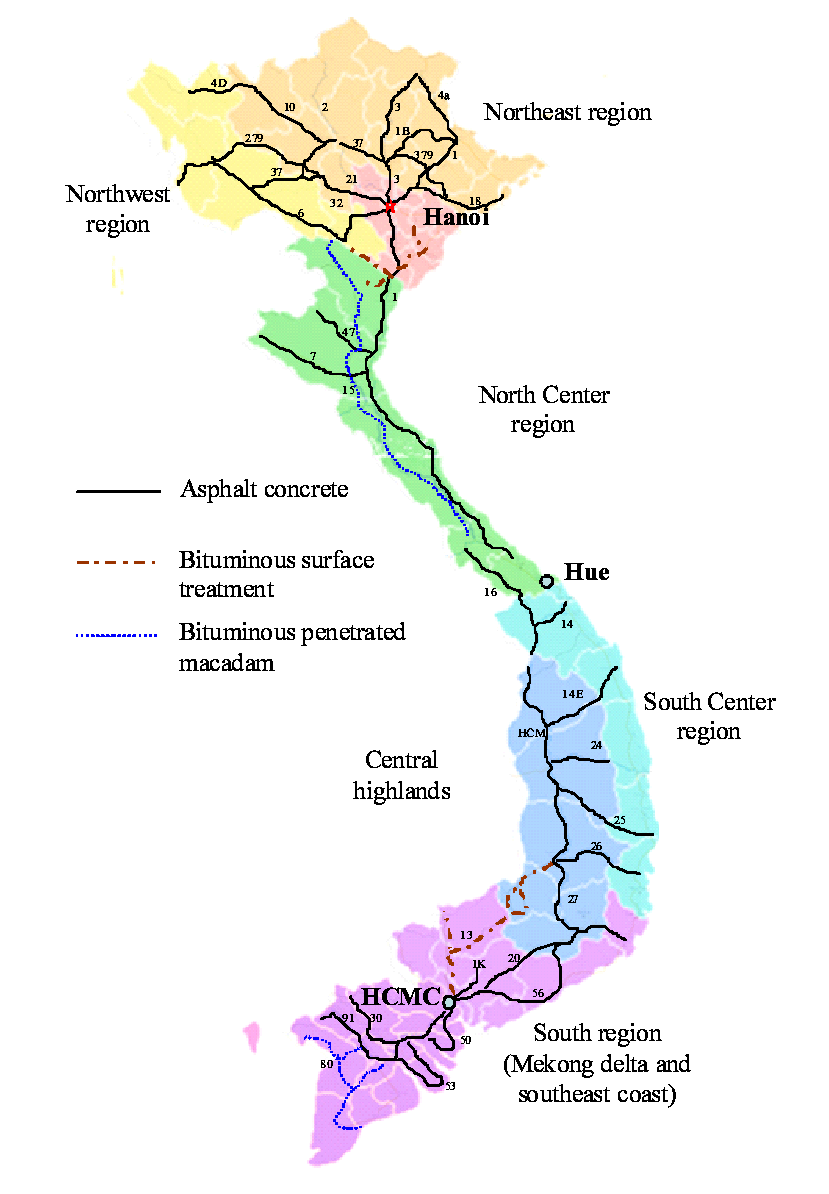
\includegraphics[scale=0.55]{fig63}
\end{center}
\caption{Repair strategy $d_1$.}
\label{fig63}
\end{figure}
%%%
\begin{table}[t]
\caption{Markov transition probability-repair strategy $d_1$.}
\label{table63}
\begin{center}
{\small
\begin{tabular}{l|lllll}
\hline
\multicolumn{1}{c|}{Condition} & \multicolumn{5}{c}{Condition state} \\ 
\multicolumn{1}{c|}{state} & \multicolumn{1}{c}{1} & \multicolumn{1}{c}{2} & \multicolumn{1}{c}{3} & \multicolumn{1}{c}{4} & \multicolumn{1}{c}{5} \\ 
\hline
\multicolumn{1}{c|}{1} & \multicolumn{1}{c}{0.4502} & \multicolumn{1}{c}{0.4965} & \multicolumn{1}{c}{0.0495} & \multicolumn{1}{c}{0.0038} & \multicolumn{1}{c}{0.0} \\ 
\multicolumn{1}{c|}{2} & \multicolumn{1}{c}{0.0017} & \multicolumn{1}{c}{0.8323} & \multicolumn{1}{c}{0.1496} & \multicolumn{1}{c}{0.0164} & \multicolumn{1}{c}{0.0} \\ 
\multicolumn{1}{c|}{3} & \multicolumn{1}{c}{0.0476} & \multicolumn{1}{c}{0.0} & \multicolumn{1}{c}{0.7983} & \multicolumn{1}{c}{0.1741} & \multicolumn{1}{c}{0.0} \\ 
\multicolumn{1}{c|}{4} & \multicolumn{1}{c}{0.2518} & \multicolumn{1}{c}{0.0} & \multicolumn{1}{c}{0.0} & \multicolumn{1}{c}{0.7482} & \multicolumn{1}{c}{0.0} \\ 
\multicolumn{1}{c|}{5} & \multicolumn{1}{c}{1.0} & \multicolumn{1}{c}{0.0} & \multicolumn{1}{c}{0.0} & \multicolumn{1}{c}{0.0} & \multicolumn{1}{c}{0.0} \\ 
\hline
\end{tabular}
}
\end{center}
\end{table}
%
\begin{figure}[t]
\begin{center}
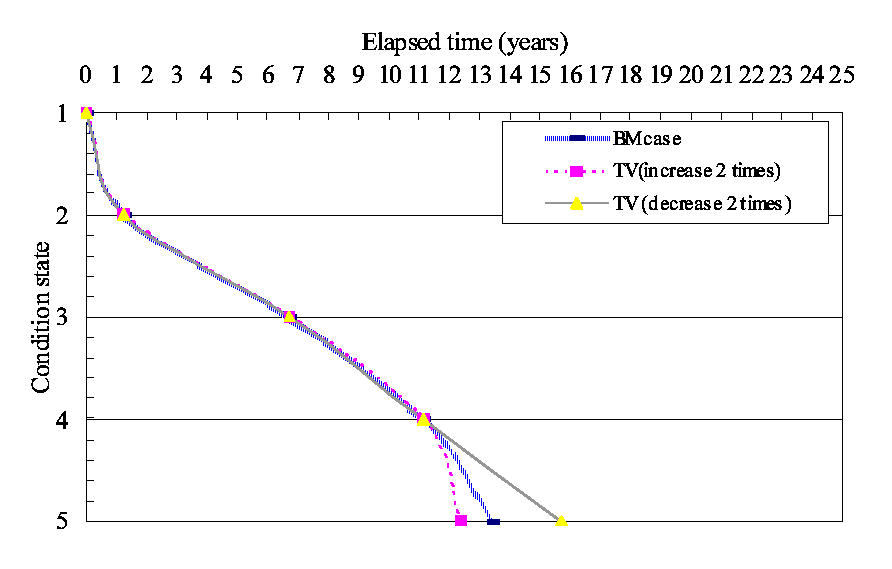
\includegraphics[scale=0.55]{fig64}
\end{center}
\caption{Repair strategy $d_2$.}
\label{fig64}
\end{figure}
%
\begin{table}[t]
\caption{Markov transition probability-repair strategy $d_2$.}
\label{table64}
\begin{center}
{\small
\begin{tabular}{l|lllll}
\hline
\multicolumn{1}{c|}{Condition} & \multicolumn{5}{c}{Condition state} \\ 
\multicolumn{1}{c|}{state} & \multicolumn{1}{c}{1} & \multicolumn{1}{c}{2} & \multicolumn{1}{c}{3} & \multicolumn{1}{c}{4} & \multicolumn{1}{c}{5} \\ 
\hline
\multicolumn{1}{c|}{1} & \multicolumn{1}{c}{0.4540} & \multicolumn{1}{c}{0.4965} & \multicolumn{1}{c}{0.0495} & \multicolumn{1}{c}{0.0} & \multicolumn{1}{c}{0.0} \\ 
\multicolumn{1}{c|}{2} & \multicolumn{1}{c}{0.0181} & \multicolumn{1}{c}{0.8323} & \multicolumn{1}{c}{0.1496} & \multicolumn{1}{c}{0.0} & \multicolumn{1}{c}{0.0} \\ 
\multicolumn{1}{c|}{3} & \multicolumn{1}{c}{0.2017} & \multicolumn{1}{c}{0.0} & \multicolumn{1}{c}{0.7983} & \multicolumn{1}{c}{0.0} & \multicolumn{1}{c}{0.0} \\ 
\multicolumn{1}{c|}{4} & \multicolumn{1}{c}{1.0} & \multicolumn{1}{c}{0.0} & \multicolumn{1}{c}{0.0} & \multicolumn{1}{c}{0.0} & \multicolumn{1}{c}{0.0} \\ 
\multicolumn{1}{c|}{5} & \multicolumn{1}{c}{1.0} & \multicolumn{1}{c}{0.0} & \multicolumn{1}{c}{0.0} & \multicolumn{1}{c}{0.0} & \multicolumn{1}{c}{0.0} \\ 
\hline
\end{tabular}
}
\end{center}
\end{table}
%
\begin{figure}[t]
\begin{center}
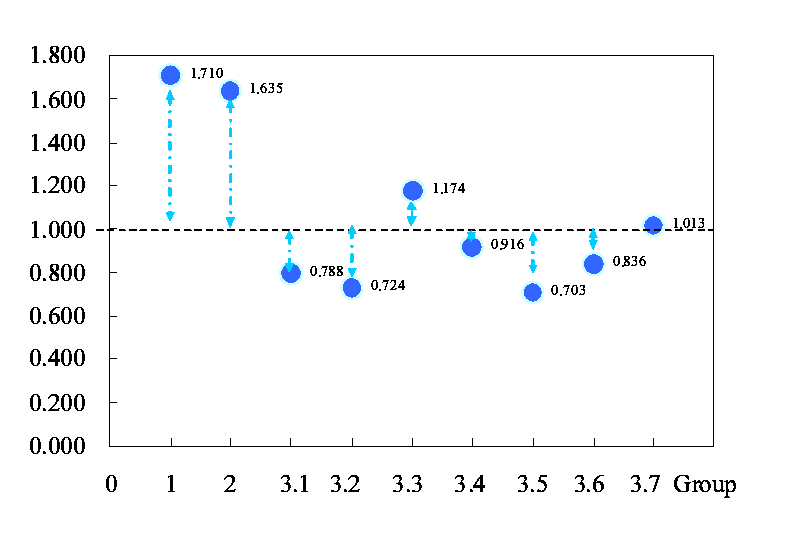
\includegraphics[scale=0.55]{fig65}
\end{center}
\caption{Repair strategy $d_3$.}
\label{fig65}
\end{figure}%
%%
\begin{table}[t]
\caption{Markv transition probability-repair strategy $d_3$.}
\label{table65}
\begin{center}
{\small
\begin{tabular}{l|lllll}
\hline
\multicolumn{1}{c|}{Condition} & \multicolumn{5}{c}{Condition state} \\ 
\multicolumn{1}{c|}{state} & \multicolumn{1}{c}{1} & \multicolumn{1}{c}{2} & \multicolumn{1}{c}{3} & \multicolumn{1}{c}{4} & \multicolumn{1}{c}{5} \\ 
\hline
\multicolumn{1}{c|}{1} & \multicolumn{1}{c}{0.5035} & \multicolumn{1}{c}{0.4965} & \multicolumn{1}{c}{0.0} & \multicolumn{1}{c}{0.0} & \multicolumn{1}{c}{0.0} \\ 
\multicolumn{1}{c|}{2} & \multicolumn{1}{c}{0.1677} & \multicolumn{1}{c}{0.8323} & \multicolumn{1}{c}{0.0} & \multicolumn{1}{c}{0.0} & \multicolumn{1}{c}{0.0} \\ 
\multicolumn{1}{c|}{3} & \multicolumn{1}{c}{1.0} & \multicolumn{1}{c}{0.0} & \multicolumn{1}{c}{0.0} & \multicolumn{1}{c}{0.0} & \multicolumn{1}{c}{0.0} \\ 
\multicolumn{1}{c|}{4} & \multicolumn{1}{c}{1.0} & \multicolumn{1}{c}{0.0} & \multicolumn{1}{c}{0.0} & \multicolumn{1}{c}{0.0} & \multicolumn{1}{c}{0.0} \\ 
\multicolumn{1}{c|}{5} & \multicolumn{1}{c}{1.0} & \multicolumn{1}{c}{0.0} & \multicolumn{1}{c}{0.0} & \multicolumn{1}{c}{0.0} & \multicolumn{1}{c}{0.0} \\ 
\hline
\end{tabular}
}
\end{center}
\end{table}
%%%%%%%%%%%
%%%
Regarding the benchmarking approach to select for the best possible M\&R strategies, it is necessary to discuss the cases where M\&R shall be applied. Needless to say, M\&R is prefer selected  when the condition of highway advances into severe deterioration. In the actual practices of pavement maintenance, it is widely accepted that localized safety and global preventive maintenance are not the suitable choices on mending for severe condition states \cite{shahin05}. Major M{\&}R for asphalt highway requires to remove the  wear layers and provide a good bonding with overlay. Several methods of construction technique in asphalt materials (cold milling, cold recycling, hot recycling and AC overlay) and the choice of thickness makes it possible to propose many Major M{\&}R alternatives.

According to the standard practice in design and construction of  asphalt concrete highway in Vietnam \cite{tcnn22}, the construction norm in maintenance and repairing\cite{dm1242} and construction unit price of Hanoi city \cite{dghanoi08}, we come up with a table of cost that relatively reflects the actual repairing cost by applying different thickness of overlay to particular condition states (refer to Table \ref{table62}). 

For simulation of the life cycle cost estimation with discount present method, we assume to use the Markov transition probability described in Table \ref{table44} of Chapter \ref{Chapter4}. In addition, three control levels for maintenance of roads are also selected. The first repair strategy $d_1$ refers to the preventive repair, which does not allow condition states to fall in condition state $5$. The directions of arrows in the Figure \ref{fig63} explains the way of repairs. By implementing the repair, as the sequent, the Markov transition probabiliy will change its properties as shown in Table \ref{table63}. Similarly, Figure \ref{fig64} and Table \ref{table64} are illustrated for the repair strategy $d_2$, which prevents condition state to reach condition state $4$ and $5$. The proactive repair action to avoid condition states of road sections to advance to condition state $3$, $4$ and $5$ is demonstrated in Figure \ref{fig65} and Table \ref{table65}.

We further realize that the load bearing capacity of highway is directly depended on structures of base, sub-based and overlay. In another word, it is well understood that the differences in thickness of overlays result in different deterioration rates. The thicker of overlay a highway has, the lower deterioration rate it would be under the same conditions of environment. Thus, life cycle cost analysis for respective thickness of overlays would enable us to select the best optimal thickness. However, due to the limitation of data, in this research, we only focus on using 5 cm thickness of overlays as major M{\&}R to apply for different condition state. 

As noted in Table \ref{table62} and Table \ref{table63}, when $i=1$, $i= 2$, the deterioration probability is low. In condition state $i=3$, the deterioration state to be faster. Thus, a localized safety and global preventive maintenance are suggested to apply as most effective. Major M{\&}R will be carried out for condition state advance from $i=3$ to $i=5$. In this understanding, the total number of major M{\&}R is 3. We notates the major M{\&}R by space vector $D=(d1,d2,d3)$, with $d1, d2, d3$ as repair actions applied to condition state $i=3$, $i=4$, and $i=5$ respectively. The horizon of one management term is assumed to be in $20$ years, the discounted factor $\delta$ equals to 0.8. Finally, result of LCC analysis for repair actions $d1, d2$ and $d3$ is calculated and displayed in Figure \ref{fig66}.

\begin{figure}[t]
\begin{center}
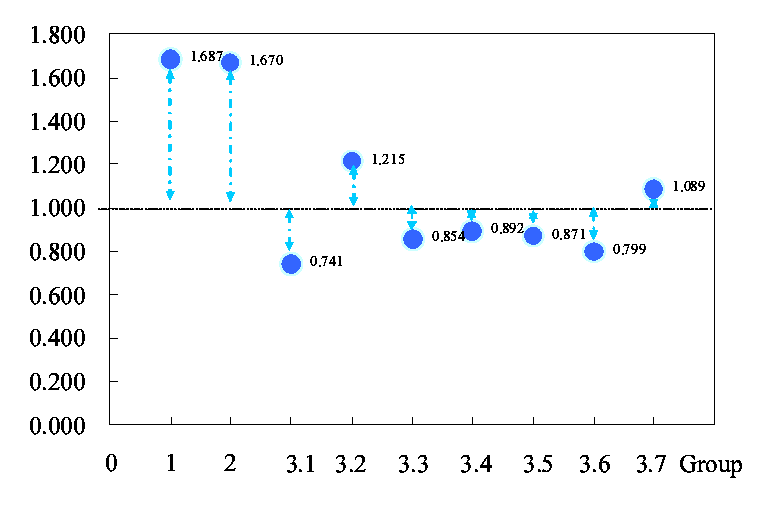
\includegraphics[scale=0.55]{fig66}
\end{center}
\caption{Deterioration curve.}
\label{fig66}
\end{figure}%
%
\begin{figure}[t]
\begin{center}
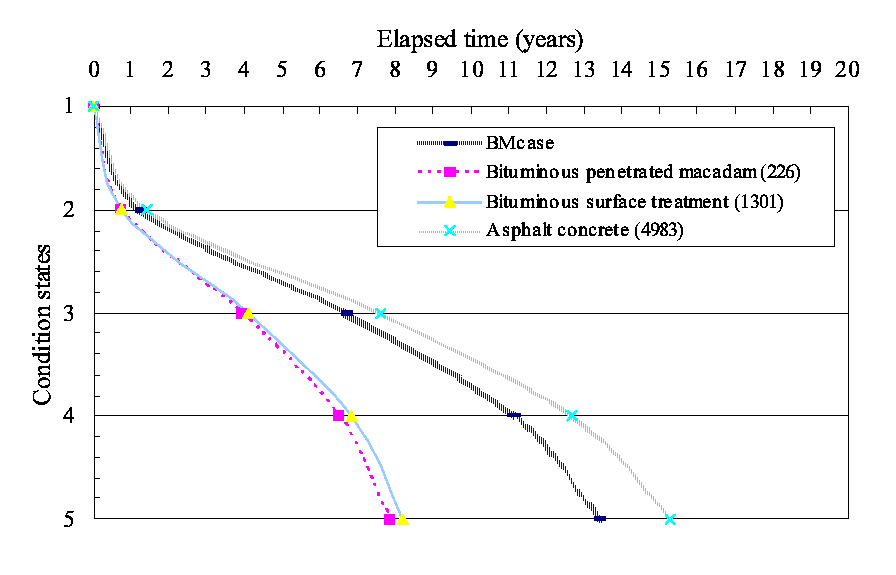
\includegraphics[scale=0.55]{fig67}
\end{center}
\caption{Deterioration curve (Case 2).}
\label{fig67}
\end{figure}%

The time horizon (or management term) can be either longer or shorter depending on the objective of investment. For this cases, the optimal repair rule in the time horizon of $20$ years is expressed by space $d^*=(d3, d3, d3, d3, d3, d3, d3,$ $d3, d3, d3, d3, d3, d3, d3, d3, d3, d3, d3, d3)$ since this rule gives the minimum expectation cost . In order to prove the effects of the repair cost on the optimal repair rules. We slightly modify the unit cost for respective repair rules as ($41.93$ for $d1$, $32.42$ for $d2$ and $29.20$ for $d3$) and obtained the different results as pointed up in Figure \ref{fig67}. For this case, the optimal repair rules alternatively becomes $d^*=(d2, d2, d2, d2, d2, d2, d2, d2, d2,$ $ d2, d2, d2, d3, d3, d3, d3, d3, d3, d3)$.

The above empirical results only demonstrate one of the possibility of applying life cycle cost model to find out the optimal M\&R technoligies. However, a detail investigation into the system compulsorily requires rigorous classification of M\&R technologies and the most up to data cost data. The emprical study remains one of the substantial problem that the classification of M\&R works in Vietnam have small scale correlation with IRI indicator. In Vietnam, as a particular case, the M\&R works are much in relation to Elastic modulus of pavement structure. However, the limitation of information on Elastic Modulus indicator from given database, in somewhat extend, prevents a deeper look into recommendations for the nation.
%%%
\section{Summary and Recommendations}
This chapter has discussed the benchmarking approach to select the best possible infrastructure technologies. Particularly, the discussion and empirical study focus on pavement system. By a simple cost evaluation technique, the best technology, which yields a minimum expected life cycle cost, can be learned. In case of benchmarking application for selection of optimal M\&R actions in operation phase of the infrastructure, a discount present cost evaluation technique, which integrated with Markov decision process, is suggested. Nevertheless, the empirical study still endures some limitation which would be considered for recommendation of future studies.
\begin{itemize}
\item This chapter focuses particularly on benchmarking model, which applies on pavement management system. However, its application can be extend to other type of infrastructure, where encounter relevant needs and sampling population.
\item This benchmarking study aims to present the possibility of using mixture hazard model for selection of asphalt materials and attempting to see the difference in deterioration speeds of road surface among regions of Vietnam. However, we have not considered the measurement error or bias, which could possible lead to less accurate estimation result.
\item This study in combination with empirical analysis of Chapter \ref{Chapter4} have captured a comparative picture of deterioration progress of asphalt roads among different climate zone in Vietnam. However, a full benchmarking study for selecting the best pavement technology for each region was not targeted due to limitation of data. It is hope that future research will encompass this important matter.
\end{itemize}